%%%%%%%%%%%%%%%%%%%%%%%%%%%%%%%%%%%%%%%%%%%%%%%%%%%%%%%%%%%%%%%%%%%%%%%%%%%%%%%
%% Chapter: Off-Policy Evaluation and Dynamic Treatment Effects
%% Section labels: section:rl_for_ci
%%
%% Structure (post 2026-07-23 split; causal bandits + adaptive experimentation
%% moved to ch10c_adaptive_experiments/tex/adaptive_experiments.tex):
%%   §1 dynamic treatment regimes (g-methods bridge)
%%   §2 DML for dynamic effects
%%   §3 dynamic offline policy learning
%%   §4 simulation studies
%%   §5 discussion
%%%%%%%%%%%%%%%%%%%%%%%%%%%%%%%%%%%%%%%%%%%%%%%%%%%%%%%%%%%%%%%%%%%%%%%%%%%%%%%

%%%%%%%%%%%%%%%%%%%%%%%%%%%%%%%%%%%%%%%%%%%%%%%%%%%%%%%%%%%%%%%%%%%%%%%%%%%%%%%
%% Chapter intro
%%%%%%%%%%%%%%%%%%%%%%%%%%%%%%%%%%%%%%%%%%%%%%%%%%%%%%%%%%%%%%%%%%%%%%%%%%%%%%%

The preceding chapter imported causal-inference machinery into reinforcement learning, asking how to recover the value of a target policy from observational data when unobserved confounders corrupt the logged transitions. This chapter reverses the direction. The question here concerns how sequential-decision methods can be used to estimate causal effects in the first place, rather than how to protect an RL estimator from confounding. The central claim is that the Bellman recursion, which underlies every RL algorithm, is the same backward induction that the causal-inference literature calls g-computation, and that recognizing this identity opens a productive two-way exchange between the fields.

The connection is older than it might appear. \citet{robins1986} introduced g-estimation to identify causal effects under time-varying confounding, and the optimal-regime problem he studied calls for exactly the kind of backward recursion that \citet{watkins1992_paper} later rediscovered independently as $Q$-learning. \citet{murphy2003dtr} made the structural link explicit, showing that the optimal dynamic treatment regime solves a finite-horizon Bellman equation identifiable from observational cohorts under sequential ignorability. The dictionary between the two traditions, translated systematically by \citet{schulte2014qlearning}, runs term for term: the blip function is the advantage, g-computation is fitted-Q evaluation, inverse-probability weighting is importance sampling, and sequential ignorability is the offline coverage condition.

Recognizing this shared structure matters because the two fields developed different tools in response to different obstacles. Causal inference developed semiparametric efficiency theory and double-robustness machinery to handle high-dimensional nuisance estimation without sacrificing parametric-rate inference on the target. Reinforcement learning developed scalable function approximation and policy-gradient methods to handle large state spaces and online interaction. The payoff from combining them is substantial. \citet{lewisSyrgkanis2021dynamicDML} apply Neyman-orthogonal cross-fitting to the Bellman recursion for structural nested mean models \citep{robins2004snmm}, delivering $\sqrt{n}$-consistent inference on dynamic treatment effects even when the nuisance regressions use black-box machine learning. \citet{sakaguchi2024dynamicpolicy} extend this to policy optimization, obtaining the first $\sqrt{n}$ welfare-regret bound for the multi-stage problem with purely nonparametric nuisances. The mechanism in both cases is the same. Doubly-robust orthogonalization removes the first-order bias from nuisance estimation errors, so the structural target inherits the parametric rate that would hold if the nuisances were known.

This chapter develops the estimation side of that exchange in three movements. The first is the g-methods bridge itself, the shared backward recursion and the dictionary it induces. The second is off-policy evaluation, the estimation of the value of a fixed target policy from logged data, where the chapter develops the estimator canon, direct methods, importance sampling, doubly robust scores, and marginalized ratios, together with its efficiency theory. The third is inference and learning at parametric rates, $\sqrt{n}$ inference on structural nested mean models via dynamic double machine learning and $\sqrt{n}$-rate policy optimization via doubly-robust backward induction. The companion design problem, in which the experimenter controls the data-collection mechanism itself, is the subject of Chapter~\ref{section:adaptive_experiments} on causal bandits and adaptive experimentation.

%%%%%%%%%%%%%%%%%%%%%%%%%%%%%%%%%%%%%%%%%%%%%%%%%%%%%%%%%%%%%%%%%%%%%%%%%%%%%%%
\subsection{Dynamic Treatment Regimes}
\label{subsec:gmethods_bridge}
\label{subsec:murphy_watkins}
%%%%%%%%%%%%%%%%%%%%%%%%%%%%%%%%%%%%%%%%%%%%%%%%%%%%%%%%%%%%%%%%%%%%%%%%%%%%%%%

In many treatment and policy settings the analyst makes a sequence of decisions, the right choice at each step depends on the subject's evolving state, and the estimation target is the decision rule itself rather than a fixed treatment level. At each of $K$ decision points the analyst observes the subject's state $S_k$ (covariates, past treatments, past responses), chooses a treatment $A_k$, and observes the next state; after the final decision a scalar outcome $Y$ is realised. The motivating example in \citet{murphy2003dtr}, used throughout this section, is the Fast Track prevention program, a randomized study targeted at children flagged for elevated behavioral problems in kindergarten,\footnote{The program was designed to prevent the emergence of conduct disorders and drug use in at-risk children.} in which the home-visiting intensity each semester was set adaptively from a six-item family-functioning score $S_j$, with low scores indicating greater need. The design team rejected a uniform schedule because ``providing too many home visits might be detrimental, increasing risk for family dependency, pejorative labeling (by self and others) and cause attrition,'' and adopted an adaptive rule. The estimation target is the rule $\pi^* = (\pi_1^*, \ldots, \pi_K^*)$ that maximises the expected outcome; a standard randomized-trial analysis recovers the marginal effect of a fixed protocol, not a rule.

\subsubsection*{Notation and identification}

Write $\bar A_k = (A_1, \ldots, A_k)$ for the treatment history through decision $k$, $\bar S_k = (S_1, \ldots, S_k)$ for the state history, and $\bar H_k = (\bar S_k, \bar A_{k-1})$ for the observed information just before decision $A_k$. For each potential treatment path $\bar a_K$, the potential outcome $Y^*(\bar a_K)$ denotes the response that would have been observed under that path \citep{rubin1978, robins1986}. A dynamic treatment regime $\pi = (\pi_1, \ldots, \pi_K)$ is a sequence of maps $\pi_k : \bar H_k \mapsto A_k$, with value $V(\pi) = \mathbb{E}[Y^*(\pi)]$ and optimization target $\pi^* \in \arg\max_\pi V(\pi)$.

Identification rests on three assumptions; Chapter~\ref{section:causal_rl} treats failure of the third. \emph{Consistency} states that $Y = Y^*(\bar A_K)$ and $S_k = S_k^*(\bar A_{k-1})$, so observed outcomes equal realized potential outcomes. \emph{Positivity} requires every action of interest to receive strictly positive probability conditional on every history that arises in the population. \emph{Sequential ignorability} requires $A_k \perp \{Y^*, S^*_{k+1}, \ldots\} \mid \bar H_k$ for every $k$, meaning the decision $A_k$ may depend on the observed history but not on unobserved factors that also affect future states and outcomes.

\subsubsection*{The backward recursion}

Under these three assumptions, the optimal value functions satisfy the finite-horizon backward recursion
\begin{align}
V_{K+1}(\bar h_{K+1}) &= Y, \label{eq:dtr_terminal}\\
Q_k(\bar h_k, a_k) &= \mathbb{E}\!\left[V_{k+1}(\bar H_{k+1}) \,\big|\, \bar H_k = \bar h_k,\ A_k = a_k\right], \label{eq:dtr_qfunc}\\
V_k(\bar h_k) &= \max_{a_k} Q_k(\bar h_k, a_k), \qquad \pi_k^*(\bar h_k) = \arg\max_{a_k} Q_k(\bar h_k, a_k). \label{eq:dtr_bellman}
\end{align}
Murphy calls $V_k$ the \emph{optimal benefit-to-go}, inverting the engineering ``optimal cost-to-go'' of \citet{bertsekas1996} since the response is to be maximized rather than minimized. The recursion is, in her words, ``a finite time version of Bellman's equation \citep{Bellman1957}.''

What separates the setting from textbook backward induction is identification. Engineering dynamic programming is given the joint distribution of states and outcomes indexed by every possible treatment path; for any candidate path the analyst can compute or simulate the resulting distribution and take expectations. Murphy's data are different. The cohort has $N$ subjects each observed once along the single realized path that the treating physician chose. For any other path that the subject did not follow, the relevant $(\bar S_K, Y)$ distribution is counterfactual and unobserved. Worse, the empirical conditional distribution of $S_{k+1}$ given $S_k$ and $A_k = a$ in the cohort is not generally the distribution of $S_{k+1}$ that would arise if every subject were assigned $a$ at stage $k$, because the decision $A_k$ may be correlated with unobserved factors that also affect $S_{k+1}$. Running the empirical Bellman backup on the cohort directly would absorb this bias into every $\hat Q_k$.

Sequential ignorability rules out the bias. Conditional on $\bar H_k$, the action $A_k$ is independent of future potential outcomes, so any factor that influences both $A_k$ and future states or outcomes must be measured in the history. The treating physician may consult anything in the chart, including past treatment responses, but does not condition on private information unavailable to the analyst. Under this assumption Robins's G-computation formula identifies the counterfactual outcome distribution from the observed-data distribution, and the recursion in \eqref{eq:dtr_qfunc}--\eqref{eq:dtr_bellman} runs empirically. Take the $K = 2$ case with binary actions to see what this looks like in practice. At stage two, $Q_2(\bar h_2, a_2) = \mathbb{E}[Y \mid \bar H_2 = \bar h_2, A_2 = a_2]$ is estimated by regressing $Y$ on $(\bar h_2, a_2)$ across the cohort, giving $\hat Q_2$ and $\hat V_2(\bar h_2) = \max_{a_2} \hat Q_2(\bar h_2, a_2)$ at every history. At stage one, $\hat V_2(\bar H_2)$ is then treated as a synthetic outcome and regressed on $(\bar h_1, a_1)$, yielding $\hat Q_1$. The optimal rule at each stage is the argmax of the corresponding regression. The whole estimator is two regressions executed in sequence. In the offline-RL literature this backward-induction-with-regression procedure is known as Fitted $Q$-Iteration \citep{Ernst2005}, and it is precisely the batch form of the Bellman backup that $Q$-learning implements online. Sections~3 and~4 of \citet{murphy2003dtr} refine the procedure by reparameterising in terms of regret contrasts, which lets the estimator place smoothness assumptions only on the quantities directly relevant for the optimal rule.

\subsubsection*{Connection to $Q$-learning and the dictionary}

The recursion in \eqref{eq:dtr_qfunc}--\eqref{eq:dtr_bellman} is the same Bellman backup that drives $Q$-learning, covered in Section~\ref{section:rl_algorithms}. \citet{watkins1992_paper} estimates $Q^*$ from a stream of $(s, a, r, s')$ transitions, with each observation nudging the current estimate by stochastic approximation. Murphy estimates the same conditional expectation in batch, with one regression per decision stage on the full cohort. The role that successive transitions play in Watkins's setting is played by successive subjects in Murphy's. Enrolling another patient adds a row to each per-stage regression and sharpens $\hat Q_k$, the way an arriving transition adjusts $\hat Q$ in $Q$-learning. A Murphy cohort replayed one subject at a time, with each $\hat Q_k$ updated by a temporal-difference step rather than refit, would converge to the same $Q^*$.

Three questions make the equivalence concrete. First, do Murphy's batch backward regression and online $Q$-learning recover the same optimal regime on a tractable two-stage DTR as the cohort size grows? Second, $Q$-learning solves the recursion by stochastic approximation rather than by one-shot regression; how does its recovered regime improve as the cohort is replayed more times at a fixed cohort size? Third, when the state is high-dimensional and tabular $Q$ is infeasible, do the neural-network analogues of the two estimators -- Neural Fitted $Q$-Iteration and DQN -- still recover the same optimal regime?

The tractable setting is a synthetic two-stage DTR with a five-level ordinal status $S_k \in \{1, \ldots, 5\}$, a binary action, a logistic behavior policy, and an outcome that rewards treatment when status is low and penalizes it when status is high. The high-dimensional setting holds the structural form fixed but replaces the five-level state with a $p = 10$-dimensional continuous one, an autoregressive transition with treatment effect on the first coordinate, and the same threshold interaction in the outcome.\footnote{Implementation source: \texttt{ch10b\_rl\_for\_ci/sims/dtr\_qlearning\_vs\_murphy.py}. Tabular case: $Q$ over the (history, action) grid for both estimators, oracle $V^*$ by exact backward induction, 50 Monte Carlo seeds. High-dimensional case: two-layer MLPs with $64$ hidden units for both estimators (Neural Fitted $Q$-Iteration fits Q stage-by-stage by full-batch MSE; DQN trains both Q networks jointly by minibatch TD), oracle $V^*$ by Monte Carlo on the known DGP, 20 Monte Carlo seeds.} Both DGPs respect sequential ignorability by construction.

Figure~\ref{fig:dtr_qlearning_vs_murphy} reports the value of the recovered regime, $V(\hat\pi) / V^*$, across the three questions. The Murphy reference baseline is implemented as saturated plug-in g-computation, the tabular form of Fitted $Q$-Iteration described above, rather than the regret/blip reparameterisation of Sections~3--4 of \citet{murphy2003dtr}.\footnote{Implementing the regret/blip estimator is straightforward but adds little to the present comparison, whose target is the recursion identity \eqref{eq:dtr_qfunc}--\eqref{eq:dtr_bellman} that batch g-computation and online $Q$-learning share. The plug-in form makes the identity most directly visible.} Panel (Q1) shows the tabular sample-size sweep. The plug-in g-computation curve and the online $Q$-learning curve overlap throughout, both approaching $V^*$ as $N$ grows; the small residual gap at large $N$ is the constant-$\alpha$ bias of $Q$-learning. Panel (Q2) shows the tabular training-budget sweep at $N = 300$. $Q$-learning at one replay epoch sits below the converged plug-in g-computation reference; by three epochs it has caught up. Panel (Q3) shows the high-dimensional sample-size sweep. Neural Fitted $Q$-Iteration and DQN both rise from the behavior-policy baseline toward $V^*$ as the cohort grows, with Neural-FQI slightly more sample-efficient at moderate $N$ because it trains the stage-two regression to convergence before bootstrapping the stage-one regression.\footnote{Neural Fitted $Q$-Iteration and DQN are not gradient-step-equated in this comparison; with $200$ full-batch epochs per stage, Neural-FQI iterates value targets across the dataset roughly four times more often than DQN with $8{,}000$ minibatch updates of size $64$ at the largest cohort. The panel-(Q3) gap therefore reflects combined sample-and-compute efficiency rather than sample efficiency alone.} The equivalence still holds under function approximation.

\begin{figure}[htbp]
\centering
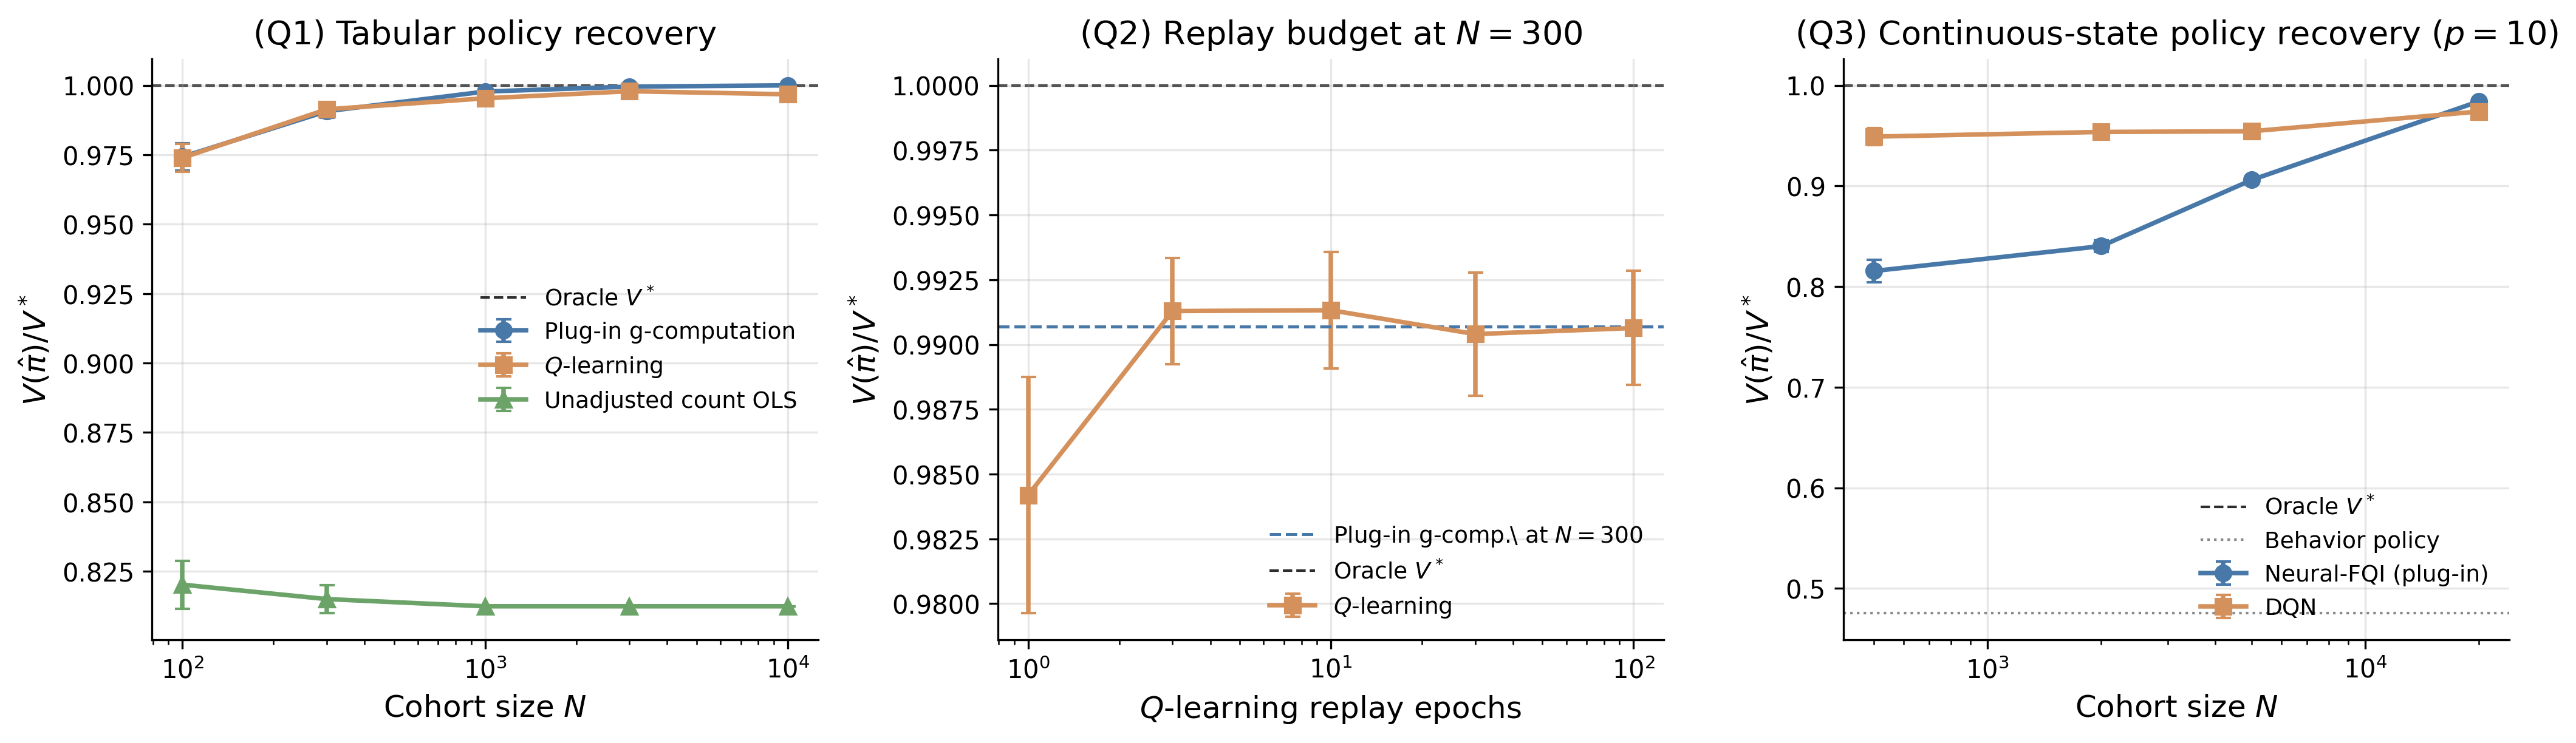
\includegraphics[width=\textwidth]{../ch10b_rl_for_ci/sims/dtr_qlearning_vs_murphy.png}
\caption{Plug-in g-computation (Murphy 2003 reference baseline) vs online $Q$-learning on a synthetic two-stage DTR under sequential ignorability. (Q1) Tabular sample-size sweep at fixed $Q$-learning budget, 50 Monte Carlo seeds, paired across estimators (both methods see the same cohort at each seed). (Q2) Tabular training-budget sweep at fixed $N = 300$, 50 seeds, with the plug-in-g-computation converged value as the dashed reference. (Q3) High-dimensional sweep ($p = 10$ continuous state), 20 seeds, paired across estimators, comparing Neural Fitted $Q$-Iteration to DQN with the same MLP architecture; the dotted line is the behavior-policy value. Error bars are 95\% confidence intervals over Monte Carlo seeds.}
\label{fig:dtr_qlearning_vs_murphy}
\end{figure}

\begin{table}[htbp]
\centering
\caption{Recovered policy value $V(\hat\pi) / V^*$ at the largest cohort size on the synthetic two-stage DTR (rank-ordered by performance). Tabular setting: $N = 10{,}000$ subjects, 50 Monte Carlo seeds, paired across the two estimators. High-dimensional setting: $p = 10$ continuous state, $N = 5{,}000$, 20 Monte Carlo seeds, paired across the two estimators.}
\label{tab:dtr_qlearning_vs_murphy}
\begin{tabular}{lcc}
\toprule
Method & $V(\hat\pi) / V^*$ & SE \\
\midrule
Murphy / FQI (tabular, $N=10000$) & 1.0000 & (0.0000) \\
Oracle $V^*$ (tabular) & 1.0000 & -- \\
Oracle $V^*$ (high-dim, $p=10$) & 1.0000 & -- \\
$Q$-learning (tabular, $N=10000$, 100 replays) & 0.9976 & (0.0006) \\
Neural-FQI / Murphy (high-dim, $N=5000$) & 0.9310 & (0.0024) \\
DQN (high-dim, $N=5000$) & 0.9126 & (0.0030) \\
\bottomrule
\end{tabular}

\end{table}

Once the Bellman recursion is shared, the rest of the vocabulary aligns predictably. Table~\ref{tab:rl_ci_dictionary} translates between the two traditions following \citet{schulte2014qlearning}.\footnote{Throughout the table, the RL state $s$ is read as the full history $\bar h_k = (\bar s_k, \bar a_{k-1})$ at decision $k$, the horizon is finite and equal to $K$, all immediate rewards are zero except $R_{K+1} = Y$, and $\gamma = 1$. The Markov property of standard RL is replaced by history augmentation.}

\begin{table}[htbp]
\centering
\caption{Translation between dynamic treatment regimes and the g-methods of \citet{robins1986, robins2000msm, murphy2003dtr, schulte2014qlearning} on the left, and reinforcement learning after \citet{watkins1992_paper, sutton2018} on the right.}
\label{tab:rl_ci_dictionary}
{\setstretch{1.0}\small
\renewcommand{\arraystretch}{1.25}
\begin{tabularx}{\textwidth}{>{\raggedright\arraybackslash}X >{\raggedright\arraybackslash}X}
\toprule
Dynamic treatment regimes / g-methods & Reinforcement learning \\
\midrule
$Q_k(\bar h_k, a_k)$, conditional mean of $V_{k+1}$ & $Q(s, a)$, state-action value function \\
$V_k(\bar h_k) = \max_{a_k} Q_k(\bar h_k, a_k)$ & $V(s) = \max_a Q(s,a)$, state value function \\
$d_k^{\text{opt}}(\bar h_k) = \arg\max_{a_k} Q_k(\bar h_k, a_k)$ & Greedy policy $\pi^*(s) = \arg\max_a Q(s,a)$ \\
Propensity $e_k(\bar h_k, a_k) = \mathbb{P}(A_k = a_k \mid \bar H_k = \bar h_k)$ & Behavior / logging policy $\mu_k(a_k \mid \bar h_k)$ \\
Value of a fixed regime $\mathbb{E}[Y^*(\pi)]$ & OPE estimand $J(\pi_e)$ (Section~\ref{subsec:ope}) \\
G-computation (sequential conditional regression) & Fitted-$Q$ evaluation \citep{Ernst2005} \\
IPTW for marginal structural models \citep{robins2000msm} & Off-policy importance sampling \citep{precup2000} \\
G-estimation for structural nested mean models \citep{robins2004snmm} & Orthogonal-score off-policy evaluation \citep{lewisSyrgkanis2021dynamicDML} \\
A-learning / contrast (blip) estimation \citep{schulte2014qlearning, robins2004snmm} & Advantage function \citep{Baird1993advantage} \\
Sequential ignorability: $A_k \perp \{Y^*, S^*_{k+1}, \ldots\} \mid \bar H_k$ & Known behavior policy $\mu_k(\cdot \mid \bar h_k)$ (offline RL setting) \\
Positivity: $e_k(\bar h_k, a) > 0$ for every action of interest & Coverage: $\mu_k(a \mid \bar h_k) > 0$ for all $a \in \mathrm{supp}\,\pi^*$ \\
\bottomrule
\end{tabularx}
}
\end{table}

Two caveats apply to the translation. First, the A-learning contrast $C_k(\bar h_k) = Q_k(\bar h_k, 1) - Q_k(\bar h_k, 0)$ is anchored at the reference action $a_k = 0$, while the RL advantage $A_k^\pi(\bar h_k, a_k) = Q_k(\bar h_k, a_k) - V_k^\pi(\bar h_k)$ is anchored at the policy mean, and the two agree only when the baseline policy is constant at $a_k = 0$. Second, sequential ignorability and the offline-RL convention of a known behavior policy play the same identification role but are not literally the same statement, the former a property of the unobserved confounder structure and the latter a property of the data-collection protocol. The current chapter takes sequential ignorability as given throughout, and Chapter~\ref{section:causal_rl} catalogues the proxy, instrumental, sensitivity, and mediator strategies that apply when it fails.

The Murphy-Watkins bridge is now being run at scale on real electronic health records. Conservative $Q$-learning has been applied to vasopressor and intravenous-fluid recommendations on MIMIC-III sepsis cohorts \citep{kaushik2022sepsiscql} and to mechanical-ventilation parameter selection on MIMIC-III intensive-care patients \citep{kondrup2023deepvent}. Cross-site policy transfer between clinical environments has been formalised as a counterfactual problem and handled with structural causal models on a sepsis simulator \citep{killian2022cftransfer}. Methodological-rigor work emphasises that na\"ive deployment is insufficient. Cross-off-policy evaluation across reward weightings identifies policies that generalise rather than overfit on intubated COVID-19 patients in the Dutch ICU Data Warehouse \citep{roggeveen2024icmrl}, and benchmark studies show that standard offline-RL algorithms degrade markedly under realistic noise, missingness, and pharmacokinetic variability \citep{luo2024dtrbench}. Inverse-constrained methods extend the framework to infer an implicit safety specification from clinician demonstrations while the survival reward is taken as given \citep{liu2024oicrl}. The deconfounding actor-critic of \citet{yin2022deconfoundingac} bakes a balancing module directly into the actor-critic learning loop, anticipating themes that recur in Chapter~\ref{section:causal_rl}.

%%%%%%%%%%%%%%%%%%%%%%%%%%%%%%%%%%%%%%%%%%%%%%%%%%%%%%%%%%%%%%%%%%%%%%%%%%%%%%%
\subsection{Off-Policy Evaluation}
\label{subsec:ope}
%%%%%%%%%%%%%%%%%%%%%%%%%%%%%%%%%%%%%%%%%%%%%%%%%%%%%%%%%%%%%%%%%%%%%%%%%%%%%%%

Before optimizing a regime, the analyst must be able to price a fixed one. \emph{Off-policy evaluation} (OPE) is the estimation of the value of a prescribed target policy from data logged under a different policy, and it is the estimation problem to which every recursion in this chapter ultimately reduces. This section develops the estimator canon under the three identification assumptions of Section~\ref{subsec:gmethods_bridge}, which are maintained throughout; the confounded case, where sequential ignorability fails, is the subject of Chapter~\ref{section:causal_rl}.

\subsubsection*{The estimand and its identification}

Fix a finite horizon $H$ and an evaluation policy $\pi_e$. The estimand is the expected cumulative reward
\begin{equation}
J(\pi_e) = \mathbb{E}_{\pi_e}\!\left[\sum_{t=1}^{H} \gamma^{t-1} R_t\right],
\label{eq:ope_estimand}
\end{equation}
where the expectation is over trajectories generated by $\pi_e$, while the data $\mathcal{D} = \{(S_t^i, A_t^i, R_t^i)_{t=1}^{H}\}_{i=1}^{n}$ consist of $n$ trajectories generated by a behavior policy $\pi_b$. Under consistency, positivity, and sequential ignorability, the change of measure from $\pi_b$ to $\pi_e$ is governed by the per-step density ratio $\rho_t = \pi_e(A_t \mid S_t)/\pi_b(A_t \mid S_t)$ and its cumulative product $\rho_{1:t} = \prod_{t'=1}^{t} \rho_{t'}$, giving the identification
\begin{equation}
J(\pi_e) = \mathbb{E}_{\pi_b}\!\left[\rho_{1:H} \sum_{t=1}^{H} \gamma^{t-1} R_t\right].
\label{eq:ope_identification}
\end{equation}
Every estimator in this section is an empirical version of Equation~\eqref{eq:ope_estimand} computed through a different intermediate object: a fitted value function, the ratios $\rho_{1:t}$, a fitted model, or a marginal state-density ratio.

The structural assumptions on the environment matter as much as the identification assumptions. \citet{ueharaShiKallus2022ope} organize the problem into a hierarchy of nested model classes: the non-Markov decision process (NMDP), where the state may be an arbitrary history; the time-varying MDP, where transitions are Markov but stage-dependent; and the time-homogeneous MDP. The hierarchy is not cosmetic. It determines which ratios an estimator must carry, and, as shown below, whether the exponential-in-horizon variance of trajectory-level weighting can be escaped at all. The contextual bandit is the $H = 1$ boundary case, where the canon originates \citep{dudik2014doubly}, and the dynamic treatment regime literature of Section~\ref{subsec:gmethods_bridge} is the same problem for longitudinal treatment policies, so DTR value estimation and OPE are one estimation problem in two vocabularies \citep{sonabend2023ssoprl, wangtom2025dtrtutorial}.

\subsubsection*{The direct method}

The \emph{direct method} (DM) estimates the conditional-mean structure and plugs it into the Bellman recursion. Its regression form is fitted-Q evaluation. Set $\hat{q}_{H+1} \equiv 0$ and, for $t = H, \ldots, 1$, regress
\begin{equation}
\hat{q}_t(s, a) \approx \widehat{\mathbb{E}}\!\left[R_t + \gamma\, \hat{q}_{t+1}(S_{t+1}, \pi_e) \mid S_t = s,\ A_t = a\right],
\qquad
\hat{J}_{\mathrm{DM}} = \frac{1}{n} \sum_{i=1}^{n} \hat{q}_1(S_1^i, \pi_e),
\label{eq:ope_dm}
\end{equation}
where $\hat{q}(s, \pi) = \sum_a \pi(a \mid s)\, \hat{q}(s, a)$. The model-based variant fits $(\hat{P}, \hat{r})$ and runs the exact recursion in the fitted model; in a tabular environment the two coincide at the maximum-likelihood estimate, and both are the g-formula plug-in of Table~\ref{tab:rl_ci_dictionary}. The direct method has low variance because no importance ratios appear, but its bias is the approximation error of the regression class, which is uncontrolled under misspecification and cannot be diagnosed from the data alone \citep{jiangli2016doubly, farajtabar2018mrdr}.\footnote{The temporal-difference family of policy evaluation algorithms, surveyed by \citet{dann2014tdsurvey} and, for the off-policy eligibility-trace variants, by \citet{geistscherrer2014traces}, supplies the incremental counterparts of the batch regression in Equation~\eqref{eq:ope_dm}.}

\subsubsection*{The importance sampling family}

\emph{Importance sampling} (IS) estimators use the ratios instead of a model. The trajectory-wise and \emph{per-decision} forms are
\begin{equation}
\hat{J}_{\mathrm{IS}} = \frac{1}{n} \sum_{i=1}^{n} \rho^i_{1:H} \sum_{t=1}^{H} \gamma^{t-1} R^i_t,
\qquad
\hat{J}_{\mathrm{PDIS}} = \frac{1}{n} \sum_{i=1}^{n} \sum_{t=1}^{H} \gamma^{t-1} \rho^i_{1:t}\, R^i_t,
\label{eq:ope_is}
\end{equation}
both unbiased for $J(\pi_e)$ when $\pi_b$ is known and positivity holds \citep{precup2000, jiangli2016doubly}. Per-decision weighting drops the ratio factors that postdate each reward, which can only reduce variance. The \emph{weighted} (self-normalized) variant divides by the realized weight mass instead of $n$: with $w_t = n^{-1} \sum_{i} \rho^i_{1:t}$, the step-wise form is $\hat{J}_{\mathrm{WIS}} = n^{-1} \sum_i \sum_t \gamma^{t-1} (\rho^i_{1:t} / w_t) R^i_t$. WIS is biased in finite samples but consistent, its variance is much smaller than that of IS, and the step-wise version is the standard point estimator of the family \citep{jiangli2016doubly, thomas2015hcope}.\footnote{Continuous action spaces break the ratio $\rho_t$ because point masses never match; \citet{kalluszhou2018continuous} replace the indicator-style ratio with a kernel-smoothed generalized propensity and characterize the induced bias-variance tradeoff in the bandwidth.}

\subsubsection*{The doubly robust family}

The direct method and importance sampling fail in complementary ways, the former through model bias and the latter through weight variance, and the \emph{doubly robust} (DR) estimator uses each to repair the other. In the bandit case,
\begin{equation}
\hat{J}_{\mathrm{DR}} = \frac{1}{n} \sum_{i=1}^{n} \left[ \hat{q}(S^i, \pi_e) + \rho^i \left( R^i - \hat{q}(S^i, A^i) \right) \right],
\label{eq:ope_dr_bandit}
\end{equation}
which is unbiased if either the outcome model $\hat{q}$ or the propensity inside $\rho$ is correct \citep{dudik2014doubly}. \citet{jiangli2016doubly} extend the construction to the sequential problem by observing that per-decision IS satisfies a backward recursion and applying the bandit correction at every stage: with $\hat{V}_{\mathrm{DR}}^{0} = 0$,
\begin{equation}
\hat{V}_{\mathrm{DR}}^{H+1-t} = \hat{V}(S_t) + \rho_t\!\left( R_t + \gamma\, \hat{V}_{\mathrm{DR}}^{H-t} - \hat{Q}(S_t, A_t) \right),
\qquad t = H, \ldots, 1,
\label{eq:ope_dr_seq}
\end{equation}
and $\hat{J}_{\mathrm{DR}}$ averages $\hat{V}_{\mathrm{DR}}^{H}$ over trajectories. Their Theorem~1 gives an exact variance decomposition showing that the $\hat{Q}$-dependent term enters only through the error $\hat{Q} - Q$, so a good value model shrinks the variance while unbiasedness survives a bad one; per-decision IS is the special case $\hat{Q} \equiv 0$. Their Theorem~3 shows that in a class of tree-structured MDPs the estimator attains the Cramér-Rao lower bound, so double robustness costs nothing asymptotically. \citet{thomasBrunskill2016magic} self-normalize the weights inside the same score to obtain the \emph{weighted doubly robust} (WDR) estimator, and blend partial-horizon WDR estimates with the model estimate by minimizing an estimated mean-squared error, the MAGIC estimator, trading a small bias for large variance reductions. \citet{farajtabar2018mrdr} close the remaining design freedom by training $\hat{Q}$ to minimize the variance of the DR estimator itself rather than a generic regression loss, the same lesson that recurs in Section~\ref{subsec:dml_dte}, that nuisances serve the target functional rather than generic prediction.

\subsubsection*{The curse of horizon and marginalized ratios}

The cumulative ratio $\rho_{1:H}$ is a product of $H$ terms, and products of ratios are asymptotically log-normal, so the variance of trajectory-level weighting grows exponentially in the horizon. This is the \emph{curse of horizon} \citep{liu2018curse}.\footnote{With a constant per-step ratio spread of $1.5$ versus $0.75$, the cumulative weight at $H = 16$ already spans eight orders of magnitude across trajectories; a handful of trajectories carry nearly all the weight and the effective sample size collapses.} \citet{xie2019marginalized} show that when the environment is a genuine MDP the trajectory ratio is unnecessary: it suffices to reweight by the \emph{marginal} state-density ratio at each stage. The marginalized importance sampling (MIS) estimator is
\begin{equation}
\hat{J}_{\mathrm{MIS}} = \frac{1}{n} \sum_{i=1}^{n} \sum_{t=1}^{H} \gamma^{t-1}\, \frac{\hat{d}^{\pi_e}_t(S^i_t)}{\hat{d}^{\pi_b}_t(S^i_t)}\, \rho^i_t\, R^i_t,
\label{eq:ope_mis}
\end{equation}
where $\hat{d}^{\pi_b}_t$ is the empirical state distribution and $\hat{d}^{\pi_e}_t$ is built by the forward recursion $\hat{d}^{\pi_e}_{t+1} = \hat{P}^{\pi_e}_t \hat{d}^{\pi_e}_t$ through a ratio-weighted empirical transition operator. Their Theorem~4.1 bounds the mean-squared error by a polynomial in $H$, matching the Cramér-Rao lower bound for the MDP class up to a factor of $H$, whereas no estimator can escape the exponential dependence in the NMDP class \citep{jiangli2016doubly}. In the infinite-horizon stationary setting the object becomes a single stationary density ratio $w(s, a)$; \citet{nachum2019dualdice} estimate it through a convex saddle-point program without knowledge of $\pi_b$, and \citet{kallusUehara2022doubleRL} combine the estimated ratio with a fitted value function in a doubly robust score that achieves the semiparametric efficiency bound under $o_p(n^{-1/4})$ nuisance rates.

\subsubsection*{Efficiency, high-confidence bounds, and estimator selection}

Semiparametric theory closes the design space. For the bandit case the efficient influence function of $J$ is $\eta(s,a)\{r - q(s,a)\} + q(s, \pi_e) - J$ with $\eta = \pi_e/\pi_b$, and the efficiency bound, the smallest asymptotic variance attainable by any regular estimator, is $\mathbb{E}[\eta^2 \operatorname{var}(R \mid S, A)] + \operatorname{var}\{q(S, \pi_e)\}$; the doubly robust estimator built from cross-fitted nuisances attains it whenever both nuisances converge at $o_p(n^{-1/4})$ rates \citep{ueharaShiKallus2022ope}. The sequential extensions replace $\eta$ by the cumulative ratio in the NMDP class and by the marginal density ratio in the MDP class, and the MDP bound is strictly smaller, which is the efficiency-theoretic statement of the marginalized escape from the horizon curse \citep{kallusUehara2022doubleRL}. The cross-fitting logic and the second-order bias structure are the same orthogonal-moment machinery as Section~\ref{subsec:dml_dte}.

Point estimation is not the whole task, because a deployment decision needs a guarantee rather than a number. \emph{High-confidence off-policy evaluation} constructs a lower confidence bound on $J(\pi_e)$ from the importance-weighted returns; the difficulty is that the weight distribution is heavy-tailed on the upside, so naive concentration inequalities are extremely loose, and \citet{thomas2015hcope} combine truncated weights with an empirical concentration argument to obtain usable bounds. \citet{sakhi2024logsmoothing} obtain tighter pessimistic estimates by logarithmic smoothing of the ratios, with bounds that remain valid for selection and learning, not only evaluation. A separate empirical literature documents that no estimator in the canon dominates: rankings flip across environments, horizons, and behavior-evaluation policy pairs \citep{voloshin2019empirical, fu2021dope}, robustness of an estimator across its own hyperparameters is itself a selection criterion \citep{saito2021robustope}, and the best estimator for one target policy is often not the best for another, motivating policy-adaptive selection rules \citep{udagawa2023pas}. The behavior of these estimators on production-scale logs, and the reliability of offline policy selection in deployed systems, are examined in Chapter~\ref{section:field_deployments}.

The simulation study of Section~\ref{subsec:simstudy} (Sim~1) exercises the canon on a tabular environment with an exact dynamic-programming oracle, verifying ground-truth recovery of every estimator, the exponential-versus-polynomial horizon behavior, and the two-sided misspecification pattern that defines double robustness.

%%%%%%%%%%%%%%%%%%%%%%%%%%%%%%%%%%%%%%%%%%%%%%%%%%%%%%%%%%%%%%%%%%%%%%%%%%%%%%%
\subsection{Dynamic Double Machine Learning for Structural Nested Mean Models}
\label{subsec:dml_dte}
%%%%%%%%%%%%%%%%%%%%%%%%%%%%%%%%%%%%%%%%%%%%%%%%%%%%%%%%%%%%%%%%%%%%%%%%%%%%%%%

Section~\ref{subsec:gmethods_bridge} established that the recursion central to g-methods and the recursion central to $Q$-learning are the same object on history-augmented data. The natural follow-up question is what happens when the nuisance functions inside that recursion (the outcome regression, the propensity score) are estimated by modern machine learning. \citet{lewisSyrgkanis2021dynamicDML} answer this question for the structural nested mean model. A Neyman-orthogonal version of Robins's g-estimation, combined with cross-fitting, delivers $\sqrt n$-consistent asymptotically normal estimates of the dynamic structural parameters, and those parameters in turn deliver off-policy evaluation at parametric rates for any target dynamic policy.

For the Fast Track cohort the structural parameter $\psi_t$ has a direct interpretation as the marginal causal effect of an additional home visit at semester $t$, holding future visits at a fixed reference level. The question of this section is what valid $\sqrt n$ inference on $\psi_1$ and $\psi_2$ requires when the outcome and propensity nuisance functions are estimated by an off-the-shelf machine learner on the longitudinal cohort, and how to convert those structural parameters into the value of any counterfactual home-visiting regime.

\subsubsection*{Structural nested mean models}

Following \citet{robins1986, robins2004snmm, schulte2014qlearning}, the conditional mean of the outcome given history admits a period-by-period decomposition. For each $t = 1, \ldots, T$, the \emph{blip function} is the marginal causal effect of the period-$t$ treatment under a fixed reference future,
\begin{multline}
\gamma_t(\bar h_t, a_t) = \mathbb{E}\!\left[Y \,\big|\, \bar H_t = \bar h_t,\, A_t = a_t,\, A_{t+1} = \cdots = A_T = 0\right] \\
{}- \mathbb{E}\!\left[Y \,\big|\, \bar H_t = \bar h_t,\, A_t = 0,\, A_{t+1} = \cdots = A_T = 0\right].
\label{eq:blip_definition}
\end{multline}
A structural nested mean model parameterizes the blip as $\gamma_t(\bar h_t, a_t) = \psi_t^{\prime} B_t(\bar h_t, a_t)$ for known basis functions $B_t$ and unknown low-dimensional parameter $\psi_t \in \mathbb{R}^d$. The full structural parameter vector $\psi^* = (\psi_1^*, \ldots, \psi_T^*)$ identifies the value of any target dynamic policy via the g-formula applied to the partialled-out outcome \citep{robins2004snmm}.

\subsubsection*{Sequential residualisation}

\citet{lewisSyrgkanis2021dynamicDML} construct cross-fitted residuals via two nuisance regressions per period, one for the outcome and one for the treatment given history. Let $\hat q_t(\bar h_t) = \widehat{\mathbb{E}}[Y \mid \bar H_t]$ and $\hat p_{j,t}(\bar h_t) = \widehat{\mathbb{E}}[A_j \mid \bar H_t]$ for $j = t, t+1, \ldots, T$, fitted by any sufficiently fast machine learner on a held-out fold. Define the residualised outcome $\tilde Y_t = Y - \hat q_t(\bar H_t)$ and the residualised treatments $\tilde A_{j,t} = A_j - \hat p_{j,t}(\bar H_t)$. The main result of \citet{lewisSyrgkanis2021dynamicDML}, their Theorem~2, is that the structural parameter $\psi_t^*$ satisfies the conditional Neyman-orthogonal moment restriction
\begin{equation}
\mathbb{E}\!\left[\Big(\tilde Y_t - \sum_{j=t}^{T} \psi_j^{*\prime}\,\tilde A_{j,t}\Big)\,\tilde A_{t,t} \,\Big|\, \bar H_t\right] = 0, \qquad t = T, T-1, \ldots, 1,
\label{eq:dynamic_dml_moment}
\end{equation}
and the resulting system is solved recursively from $t = T$ downward. The algorithm estimates $\hat\psi_T$ from the period-$T$ moment, peels off the estimated period-$T$ effect from the outcome to define the calibrated outcome $\tilde Y_{T-1} - \hat\psi_T^{\prime}\,\tilde A_{T,T-1}$, regresses against $\tilde A_{T-1, T-1}$ to obtain $\hat\psi_{T-1}$, and continues backward to $\psi_1$. Each stage solves an ordinary least squares regression on residualised data.

\subsubsection*{Asymptotic normality at $\sqrt n$ rates}

The Neyman-orthogonal moment in Equation~\eqref{eq:dynamic_dml_moment} has the crucial property that small errors in the nuisance estimates $\hat q_t$ and $\hat p_{j,t}$ enter the estimating equation at second order rather than first. Theorem~4 of \citet{lewisSyrgkanis2021dynamicDML} shows that if each cross-fitted nuisance achieves mean-squared-error rate $o_p(n^{-1/4})$ in the population norm, then the recursive estimator $\hat\psi$ is $\sqrt n$-consistent and asymptotically normal,
\begin{equation}
\sqrt{n}\,(\hat\psi - \psi^*) \xrightarrow{d} \mathcal{N}(0,\, V),
\label{eq:dynamic_dml_clt}
\end{equation}
with a consistently estimable covariance matrix $V$. The $o_p(n^{-1/4})$ condition is satisfied by Lasso regression under standard sparsity conditions, by random forests under regularity conditions on the population regression function, and by any other learner that achieves the corresponding excess-risk rate. The history $\bar H_t$ may itself be high-dimensional; only the structural parameter $\psi^* \in \mathbb{R}^{Td}$ is required to be low-dimensional. The resulting confidence intervals are asymptotically uniformly valid over the corresponding class of data-generating processes.

\subsubsection*{The off-policy evaluation bridge}

The structural parameters $\psi^*$ identify the value of any target dynamic policy $\pi$, the estimand $J(\pi)$ of Section~\ref{subsec:ope}, because the SNMM blip representation gives a closed-form expression for the policy value $V(\pi) = \mathbb{E}[Y^*(\pi)]$ that depends only on $\psi^*$ and the marginal action distribution under $\pi$ \citep[Section~6]{lewisSyrgkanis2021dynamicDML}. Where the estimators of Section~\ref{subsec:ope} target $J(\pi)$ nonparametrically, the SNMM route buys the parametric rate by restricting the blip to a low-dimensional form. The headline claim from the paper's abstract states the bridge directly:
\begin{quote}
\itshape
These structural parameters can be used for off-policy evaluation of any target dynamic policy at parametric rates, subject to semi-parametric restrictions on the data generating process.
\end{quote}
This is the bridge promised at the close of Section~\ref{subsec:gmethods_bridge}. Murphy's $Q$-recursion estimated under semiparametric efficiency gives parametric-rate inference on policy value, even when the controls inside the recursion are estimated by black-box machine learning. The simulation study in Section~\ref{subsec:simstudy} demonstrates the empirical $\sqrt n$ coverage on a two-stage SNMM. At $n = 4000$, Dynamic DML attains $96.5\%$ empirical coverage of nominal $95\%$ confidence intervals on $\psi_1$ and $93.0\%$ on $\psi_2$, with RMSE shrinking at the rate predicted by Theorem~4 of \citet{lewisSyrgkanis2021dynamicDML}. The naive panel regression that omits the time-varying confounder carries a bias of $-0.19$ on $\psi_1$ and $+0.93$ on $\psi_2$ that does not shrink with the sample size, and its confidence intervals cover the truth in $1\%$ and $0\%$ of replications respectively. MSM with stabilised inverse-probability weighting is consistent but slow; at the same sample size its coverage is $88\%$ on $\psi_1$ and $73\%$ on $\psi_2$.

\subsubsection*{Recursive Riesz representers}

The Neyman-orthogonal moment of \citet{lewisSyrgkanis2021dynamicDML} is hand-derived. The residual-on-residual construction in Equation~\eqref{eq:dynamic_dml_moment} achieves orthogonality by inspection, because residualising both sides of a regression makes the moment locally insensitive to small perturbations in the nuisance regressions. \citet{chernozhukov2023automatic} automate this step. Rather than write the orthogonal moment in closed form, they characterize the de-biasing correction as a sequence of \emph{Riesz representers} solving a system of recursive linear functional equations, and they show that these representers can be learned by minimising a sequence of quadratic Riesz losses without ever writing the orthogonal moment in closed form. Formally, define $f_{T+1}(\bar h_{T+1}) = Y$ and the nested mean regressions $f_t(\bar h_t, a_t) = \mathbb{E}\!\left[f_{t+1}\bigl(\bar H_{t+1}, \pi_{t+1}(\bar H_{t+1})\bigr) \mid \bar H_t, A_t = a_t\right]$ for $t = T, \ldots, 1$. The policy value $\theta(\pi) = \mathbb{E}[Y^*(\pi)]$ admits the debiased representation
\begin{equation}
\theta(\pi) = \mathbb{E}\!\left[f_1\bigl(\bar H_1, \pi_1(\bar H_1)\bigr) + \sum_{t=1}^{T} \alpha_{t-1}(\bar H_{t-1}, A_{t-1})\,\bigl(f_{t+1}(\bar H_{t+1}, \pi_{t+1}) - f_t(\bar H_t, A_t)\bigr)\right],
\label{eq:cnss_riesz}
\end{equation}
where $\alpha_0 \equiv 1$ and each $\alpha_t : \mathcal{H}_t \times \mathcal{A}_t \to \mathbb{R}$ is the Riesz representer of the linear functional $L_t(g) = \mathbb{E}\bigl[\alpha_{t-1}(\bar H_{t-1}, A_{t-1})\,g(\bar H_t, \pi_t)\bigr]$. Each $\alpha_t$ is estimated by minimising the quadratic Riesz loss $\mathbb{E}_n\bigl[\alpha^2(\bar H_t, A_t) - 2\,\hat\alpha_{t-1}(\bar H_{t-1}, A_{t-1})\,\alpha(\bar H_t, \pi_t)\bigr]$, with no closed-form inverse-propensity-weight expression required. The two constructions are complementary. \citet{lewisSyrgkanis2021dynamicDML} target the SNMM blip parameters at parametric rates; \citet{chernozhukov2023automatic} target the policy value $\theta(\pi)$ non-parametrically. Both achieve the mixed-bias product structure under which $o_p(n^{-1/4})$ nuisance error suffices for the target oracle rate.\footnote{The reason this works at the population-risk level is the orthogonal statistical learning theory of \citet{fosterSyrgkanis2023orthogonal}, whose Theorem~1 shows that under prediction-space strong convexity of the target loss and Neyman orthogonality of the loss derivative, the excess risk of a two-stage cross-fitted estimator has nuisance error entering at second order, so $n^{-1/4}$ mean-squared error on each nuisance suffices for the target oracle rate $n^{-1}$.}

In offline-RL vocabulary, the Lewis-Syrgkanis estimator is the orthogonal-score version of fitted-Q evaluation (Section~\ref{subsec:ope}), with the residual-on-residual moment in Equation~\eqref{eq:dynamic_dml_moment} replacing the ordinary mean-squared-error loss that FQE uses to fit the period-$t$ value function. The recursive Riesz representer construction of \citet{chernozhukov2023automatic} is automatic debiased off-policy evaluation, applicable to any estimator of Section~\ref{subsec:ope} that targets a smooth functional of a sequence of conditional means, including fitted-Q evaluation, model-based OPE, and marginalised importance sampling. The bridge in this section is what lets those RL OPE methods inherit the $\sqrt n$ rate that semiparametric efficiency theory establishes for the SNMM target.

%%%%%%%%%%%%%%%%%%%%%%%%%%%%%%%%%%%%%%%%%%%%%%%%%%%%%%%%%%%%%%%%%%%%%%%%%%%%%%%
\subsection{Dynamic Offline Policy Learning}
\label{subsec:dynamic_offline_policy}
%%%%%%%%%%%%%%%%%%%%%%%%%%%%%%%%%%%%%%%%%%%%%%%%%%%%%%%%%%%%%%%%%%%%%%%%%%%%%%%

Section~\ref{subsec:dml_dte} delivers $\sqrt n$ confidence intervals on dynamic structural parameters under sequential ignorability, which in turn deliver off-policy evaluation at parametric rates for any target dynamic policy. This subsection turns from evaluation to optimization. Given observational data on $n$ trajectories, can we \emph{learn} an optimal dynamic regime $\pi^* \in \arg\max_{\pi \in \Pi} V(\pi)$ at the same $\sqrt n$ regret rate, using modern machine learning for the nuisances? \citet{sakaguchi2024dynamicpolicy} answers yes, by combining the doubly-robust AIPW machinery of \citet{athey2021policy} with fitted-$Q$-evaluation in a backward-induction loop.

For the Fast Track cohort, a natural restricted policy class is the family of threshold rules in the family-functioning score, $\pi_t(\bar h_t) = \mathbb 1\{S_{t,j} < c_t\}$ for thresholds $(c_1, c_2)$ to be learned from data. The question of this section is the welfare-maximising thresholds with a $\sqrt n$-rate welfare-regret guarantee, when the cohort is observational and the nuisances are estimated by machine learning.

\subsubsection*{The static $T=1$ precursor}

In the single-period treatment-choice problem the offline policy-learning literature is well-developed. \citet{kitagawa2018who} introduced empirical welfare maximization with known propensities and proved a matching minimax bound of $\Theta(\sqrt{\mathrm{VC}(\Pi)/n})$ on welfare regret, applied to the National JTPA Study. \citet{athey2021policy} generalized to unknown propensities via cross-fitted doubly-robust scores (their Equation~14), maintaining the $O_p(\sqrt{\mathrm{VC}(\Pi)/n})$ rate under product-rate nuisance conditions and extending to instrumental-variable identification. \citet{zhou2023offline} extended further to multi-action treatments with an exact decision-tree-search algorithm. All three are the $T = 1$ special case of what follows.

\subsubsection*{Backward-induction AIPW under sequential ignorability}

For each stage $t = 1, \ldots, T$, fix a policy class $\Pi_t$ over which to optimize the stage-$t$ rule, and let $\Pi = \Pi_1 \times \cdots \times \Pi_T$. Define the action-value function for any candidate future policy $\pi_{(t+1):T} = (\pi_{t+1}, \ldots, \pi_T)$ recursively by
\begin{equation}
Q^{\pi_{(t+1):T}}_t(\bar h_t, a_t) = \mathbb{E}\!\left[Y_t + Q^{\pi_{(t+2):T}}_{t+1}\bigl(\bar H_{t+1}, \pi_{t+1}(\bar H_{t+1})\bigr) \,\Big|\, \bar H_t = \bar h_t, A_t = a_t\right],
\label{eq:sakaguchi_q}
\end{equation}
with terminal condition $Q_T(\bar h_T, a_T) = \mathbb{E}[Y_T \mid \bar H_T = \bar h_T, A_T = a_T]$. The recursion estimates Q in the form of \emph{fitted-Q-evaluation} \citep{Ernst2005} applied under sequential ignorability. Let $e_t(\bar h_t, a_t) = \mathbb{P}(A_t = a_t \mid \bar H_t = \bar h_t)$ denote the stage-$t$ propensity.

\citet{sakaguchi2024dynamicpolicy} estimates the optimal regime $\hat\pi = (\hat\pi_1, \ldots, \hat\pi_T)$ by backward induction with cross-fitted nuisances. Randomly partition the data into $K$ folds, and let $\hat Q^{-k}_t$ and $\hat e^{-k}_t$ denote the nuisance estimators fitted on the complement of the $k$-th fold (any sufficiently fast machine learner). Starting at $t = T$, construct the cross-fitted AIPW score for any candidate stage-$T$ policy $\pi_T$,
\begin{equation}
\hat\Gamma_{i, T}(a) = \hat Q^{-k(i)}_T(\bar H_{i,T}, a) + \frac{\mathbb 1\{A_{i,T} = a\}}{\hat e^{-k(i)}_T(\bar H_{i,T}, a)}\,\bigl(Y_{i,T} - \hat Q^{-k(i)}_T(\bar H_{i,T}, A_{i,T})\bigr),
\label{eq:sakaguchi_aipw}
\end{equation}
and select $\hat\pi_T = \arg\max_{\pi_T \in \Pi_T} \tfrac{1}{n}\sum_{i=1}^n \hat\Gamma_{i,T}(\pi_T(\bar H_{i,T}))$. Given $\hat\pi_T$, refit $\hat Q^{\hat\pi_T}_{T-1}$ by fitted-$Q$-evaluation against the calibrated next-stage value, build the stage-$T{-}1$ AIPW score from Equation~\eqref{eq:sakaguchi_aipw} with the new $Q$-function in the position of $\hat Q^{-k(i)}_T$, and select $\hat\pi_{T-1}$. Continue backward to $\hat\pi_1$. Each stage solves a single classification-style policy optimization on cross-fitted scores; the nuisances at stage $t$ depend only on the previously estimated future policies $\hat\pi_{(t+1):T}$, never on the candidate $\pi_t$ being optimized.

\subsubsection*{The $\sqrt n$ welfare regret bound}

\citet[Theorem~4.3]{sakaguchi2024dynamicpolicy} establishes that under sequential ignorability, overlap (Assumption~2.3 of the paper), a correct-specification condition on the policy classes (Assumption~3.1), uniform MSE convergence of $o_p(n^{-1/4})$ on both the $Q$-functions for the estimated future policies and the propensity scores, and an entropy-integral complexity bound on $\Pi$, the welfare regret of the estimated regime satisfies
\begin{equation}
V(\pi^*) - V(\hat\pi) = O_p\!\left(\kappa(\Pi)\, n^{-1/2}\right),
\label{eq:sakaguchi_regret}
\end{equation}
where $\kappa(\Pi)$ is the entropy integral of the DTR class. This matches the $\sqrt n$ minimax-optimal rate that \citet{kitagawa2018who} established for the static $T=1$ case, and is the first such result for the multi-stage problem with purely nonparametric ML nuisances. A companion result (their Theorem~5.1) shows that the alternative simultaneous-optimization approach attains the same rate without requiring correct specification of the policy class, at the cost of computational tractability that degrades quickly in $T$.

\subsubsection*{Empirical application}

\citet[Section~7]{sakaguchi2024dynamicpolicy} applies the method to the Tennessee Project STAR class-size experiment. The treatment at each of two stages (kindergarten, first grade) is the choice between a regular-size class with a full-time teacher aide and a small-size class without one; the welfare objective is the percentile rank of combined reading and mathematics test scores at the end of first grade. Decision trees of depth one and two are used for the stage-specific policy classes, with cross-fitted random-forest nuisances. The estimated optimal dynamic regime improves academic achievement by approximately 8\% relative to uniformly assigning all students to classes with a teacher aide, and by approximately 1\% relative to uniformly assigning to small classes, both estimated via five-fold cross-validation. A companion field experiment in Japan \citep{idaIshiharaItoEtAl2024energyrebate} applies a related dynamic-targeting estimator to energy-saving rebate programs and confirms empirically that two-period dynamic targeting outperforms one-shot static targeting on realized welfare gains.\footnote{A parallel literature targets related aspects of the same problem. \citet{nie2021whentotreat} develop an advantage doubly-robust estimator for the ``when-to-treat'' subclass of dynamic regimes and prove the first dynamic analog of the \citet{athey2021policy} static regret bound. \citet{shi2024seal} extend to infinite-horizon offline reinforcement learning, showing that the advantage function is smoother than the $Q$-function and yielding a strictly faster minimax rate than fitted-$Q$-iteration. \citet{luckett2020vlearning} introduce $V$-learning for infinite-horizon mobile-health regimes, bypassing $Q$-estimation by directly optimizing the value function via the Bellman estimating equation.}

In offline-RL vocabulary, the Sakaguchi estimator is the doubly-robust analog of \emph{fitted-Q iteration} for policy optimisation. The action-value recursion in Equation~\eqref{eq:sakaguchi_q} is fitted-Q evaluation under sequential ignorability; the augmentation in Equation~\eqref{eq:sakaguchi_aipw} adds the importance-weighted residual correction that makes the score estimator doubly robust. The connection extends downstream. \citet{shi2024seal} target the advantage function directly rather than the action-value function and obtain a faster minimax rate, in the same spirit that \emph{advantage-weighted regression} and \emph{implicit Q-learning} replace the $Q$-function with smoother surrogates for offline policy improvement. The DR-AIPW scoring is the principal innovation that distinguishes the Sakaguchi guarantee from those purely-RL offline methods, which lack the doubly-robust property and so require correct specification of either the outcome model or the propensity to attain the parametric rate.

%%%%%%%%%%%%%%%%%%%%%%%%%%%%%%%%%%%%%%%%%%%%%%%%%%%%%%%%%%%%%%%%%%%%%%%%%%%%%%%
\subsection{Simulation Studies}
\label{subsec:simstudy}
%%%%%%%%%%%%%%%%%%%%%%%%%%%%%%%%%%%%%%%%%%%%%%%%%%%%%%%%%%%%%%%%%%%%%%%%%%%%%%%

This subsection presents two computational experiments that ground the chapter's central claims. The first targets Section~\ref{subsec:ope}. On a tabular environment with an exact dynamic-programming oracle, the OPE estimator canon recovers the true policy value, trajectory-level importance sampling degrades exponentially in the horizon while the marginalized estimator does not, and the doubly robust estimator survives single-sided nuisance misspecification. The second targets Section~\ref{subsec:dml_dte}. Dynamic double machine learning on a two-stage structural nested mean model delivers $\sqrt n$ confidence intervals on the dynamic treatment effect parameters, while a naive panel regression and a marginal-structural-model with stabilized inverse-probability-of-treatment weights both fail.

\subsubsection*{Sim 1: the OPE estimator canon on a tabular retention MDP}

The environment is a promotional-targeting problem in customer retention. A customer occupies an engagement state $s \in \{0, \ldots, 4\}$, the firm holds or promotes, $a \in \{0, 1\}$, and engagement drifts up with probability $0.15$ ($0.45$ under promotion), down with probability $0.30$ ($0.15$), clipped at the boundaries. The per-period profit is $r(s, a) = 0.25\, s - 0.5 \cdot \mathbbm{1}\{a = 1\}(1 - 0.1\, s)$, margin increasing in engagement with a promotion cost partially offset for loyal customers, and $\gamma = 1$ over horizon $H$. The behavior policy promotes with probability $\pi_b(1 \mid s) = 0.6 - 0.1\, s$; the evaluation policy targets promotions at low-engagement customers, $\pi_e(1 \mid s) = 0.9$ for $s \le 1$ and $0.1$ otherwise, so the single-step ratio $\rho_t$ ranges over $[0.2, 1.8]$. The truth $J(\pi_e)$ is computed by exact backward induction at every horizon (at $H = 16$, $J(\pi_e) = 5.611$; a $100{,}000$-episode on-policy simulation agrees within $1.2$ standard errors), and all seven estimators of Section~\ref{subsec:ope} score the same logged datasets in each of $500$ Monte Carlo replications.\footnote{Sim 1 source: \texttt{ch10b\_rl\_for\_ci/sims/ope\_estimators.py}. DM fits the tabular maximum-likelihood model and solves the fitted recursion, which coincides with fitted-Q evaluation in this environment; DR and WDR use two-fold cross-fitting for $\hat Q$, with the WDR weights self-normalized within each scoring fold; MIS follows the forward recursion of \citet{xie2019marginalized}. MAGIC and DualDICE are omitted, as their blending and saddle-point machinery adds nothing qualitative on a tabular problem with an exact oracle.}

Table~\ref{tab:simA_ope} and Figure~\ref{fig:simA_ope} report the results of three experiments. In the sample-size sweep at $H = 16$, IS and PDIS are unbiased at every $n$ (bias within Monte Carlo error of zero), WIS carries a finite-sample bias that shrinks from $+0.63$ at $n = 50$ to $+0.05$ at $n = 2000$, and every estimator's RMSE falls at the $n^{-1/2}$ rate; at $n = 2000$ the ranking is DM ($0.111$), MIS ($0.214$), WDR ($0.330$), DR ($0.366$), WIS ($0.460$), PDIS ($0.601$), IS ($1.555$). The direct method wins here because the tabular model class is correctly specified by construction; the misspecification experiment below is its counterweight. In the horizon sweep at $n = 500$, the relative RMSE of IS grows from $0.09$ at $H = 4$ to $2.85$ at $H = 64$ and PDIS reaches $2.05$, while MIS grows only from $0.06$ to $0.13$, a $21$-fold separation from IS at the longest horizon, the curse of horizon and its marginalized escape \citep{liu2018curse, xie2019marginalized}. In the $2 \times 2$ misspecification design at $H = 16$, $n = 500$ (Table~\ref{tab:simA_ope_dr}), the action-pooled outcome model erases the treatment channel and the flat propensity $\tilde\pi_b = 0.5$ corrupts the ratios. DR remains unbiased when either nuisance is correct (bias $-0.03$, $-0.02$, $+0.08$ across the three one-sided cells) and breaks only when both fail ($+1.71$); DM is biased whenever its model is wrong ($+0.38$) regardless of the propensity, and PDIS is biased whenever the propensity is wrong ($+79.1$) regardless of the model, the two-sided failure pattern that Equation~\eqref{eq:ope_dr_bandit} is built to avoid.

\begin{table}[htbp]
\centering
\caption{Sim 1, OPE estimators on the tabular retention MDP. Bias, standard deviation, and RMSE of $\hat J(\pi_e)$ at $n = 2000$, $H = 16$ (truth $J(\pi_e) = 5.611$), and relative RMSE at $H = 64$, $n = 500$; 500 Monte Carlo replications, rows rank-ordered by RMSE.}
\label{tab:simA_ope}
\begin{tabular}{lrrrr}
\toprule
Estimator & Bias & SD & RMSE & Rel. RMSE at $H=64$ \\
\midrule
DM & +0.0024 & 0.1113 & 0.1112 & 0.026 \\
MIS & +0.0061 & 0.2137 & 0.2136 & 0.134 \\
WDR & -0.0181 & 0.3438 & 0.3439 & 0.209 \\
DR & -0.0179 & 0.3661 & 0.3661 & 1.242 \\
WIS & +0.0490 & 0.4580 & 0.4601 & 0.286 \\
PDIS & +0.0029 & 0.6013 & 0.6007 & 2.055 \\
IS & +0.1325 & 1.5511 & 1.5552 & 2.847 \\
\bottomrule
\end{tabular}

\end{table}

\begin{table}[htbp]
\centering
\caption{Sim 1, double-robustness ablation at $H = 16$, $n = 500$. Bias and RMSE of $\hat J(\pi_e)$ when the outcome model (action-pooled projection) and the propensity (flat $0.5$) are each correct or misspecified; DM and PDIS rows anchor the two single-nuisance estimators. 500 Monte Carlo replications.}
\label{tab:simA_ope_dr}
\begin{tabular}{lllrr}
\toprule
Estimator & $\hat Q$ model & Propensity & Bias & RMSE \\
\midrule
DR & right & right & -0.0254 & 0.7643 \\
DR & wrong & right & -0.0214 & 0.7805 \\
DR & right & wrong & +0.0771 & 6.4246 \\
DR & wrong & wrong & +1.7061 & 7.8574 \\
DM & right & -- & +0.0011 & 0.2077 \\
DM & wrong & -- & +0.3769 & 0.4128 \\
PDIS & -- & right & -0.0627 & 1.1428 \\
PDIS & -- & wrong & +79.1185 & 86.6760 \\
\bottomrule
\end{tabular}

\end{table}

\begin{figure}[htbp]
\centering
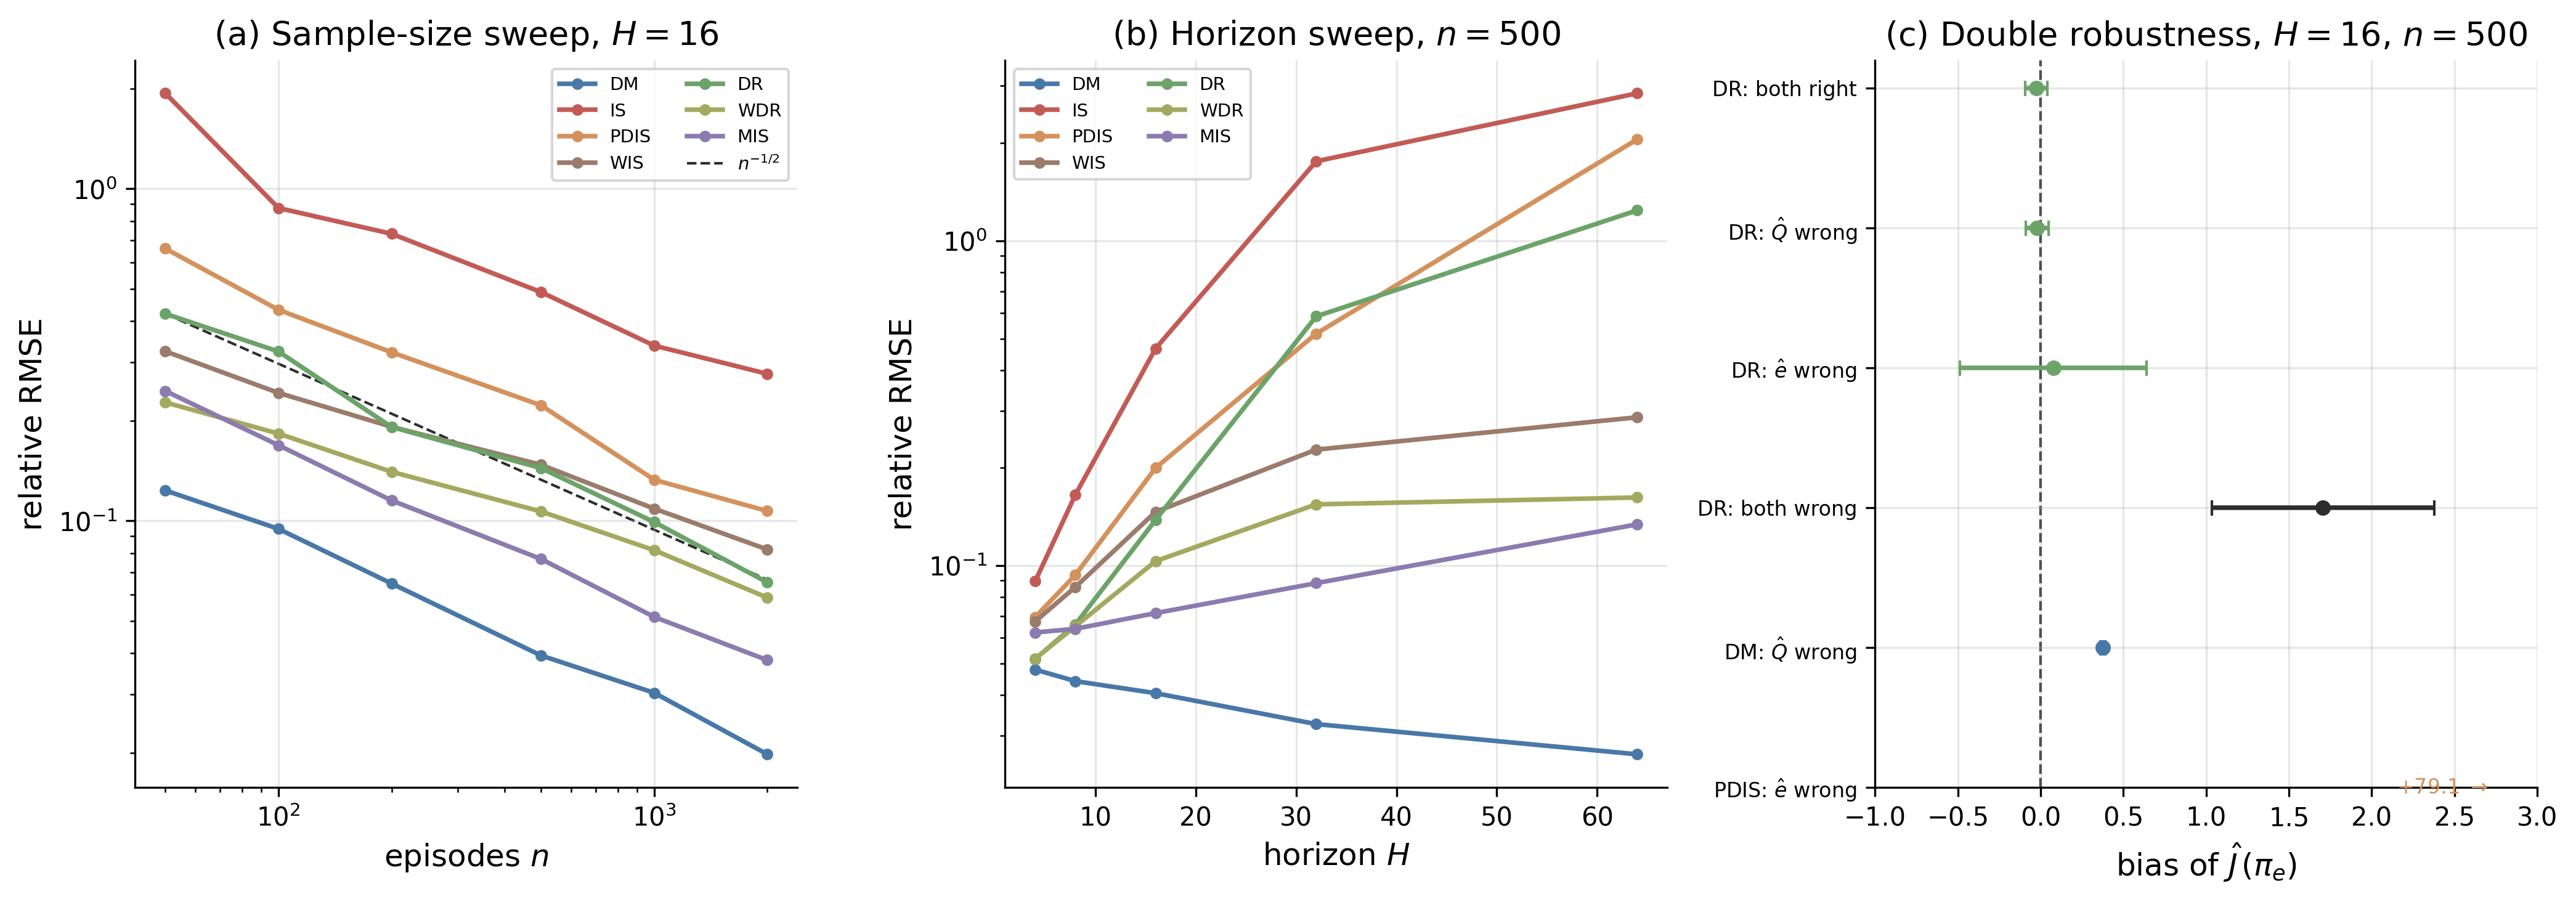
\includegraphics[width=\textwidth]{../ch10b_rl_for_ci/sims/ope_estimators.png}
\caption{Sim 1, OPE estimators on the tabular retention MDP. (a) Relative RMSE versus the number of logged episodes $n$ at $H = 16$, log-log; the dashed reference line is the $n^{-1/2}$ rate. (b) Relative RMSE versus horizon $H$ at $n = 500$, log scale. (c) Bias of $\hat J(\pi_e)$ in the double-robustness ablation with 95\% confidence whiskers; the off-scale PDIS point is annotated at the clipped axis edge. 500 Monte Carlo replications throughout.}
\label{fig:simA_ope}
\end{figure}

\subsubsection*{Sim 2: dynamic DML on a 2-stage SNMM}

The data-generating process follows a two-stage Markovian setup with high-dimensional state, confounded propensities, and treatment-confounder feedback. State dimension $p = 20$ with sparse outcome coefficients on $s = 5$ coordinates. At stage one, $X_1 \sim \mathcal{N}(0, I_p)$ and the binary treatment $T_1 \sim \mathrm{Bernoulli}(\sigma(\gamma^\top X_1))$ with $\|\gamma\|_2 = 1.5$ supported on the first $s$ coordinates. The period-1 state shock $\eta_1 \sim \mathcal{N}(0, \sigma_\eta^2 I_p)$ with $\sigma_\eta = 0.6$ drives the next state $X_2 = B X_1 + \alpha T_1 + \eta_1$ with $\|B\|_{\mathrm{op}} = 0.5$ and $\alpha = e_1$, after which $T_2 \sim \mathrm{Bernoulli}(\sigma(\gamma^\top X_2))$. The outcome
\begin{equation}
Y = \psi_1^* T_1 + \psi_2^* T_2 + \mu^\top X_1 + \nu^\top \eta_1 + \varepsilon, \qquad \varepsilon \sim \mathcal{N}(0, 0.5^2),
\label{eq:simB1_dgp}
\end{equation}
has true structural parameters $(\psi_1^*, \psi_2^*) = (1.0, 0.5)$ and the outcome-coupling vector $\nu = 2.0 \cdot \gamma / \|\gamma\|$ is aligned with the propensity direction, so that $\eta_1$ enters $Y$ and also drives the period-2 propensity through $X_2$. This is the canonical treatment-confounder-feedback channel: conditional on $(X_1, T_1)$, $T_2$ is correlated with $Y$'s residual through $\eta_1$.

Three estimators are compared. \emph{Naive OLS} regresses $Y$ on $(T_1, T_2, X_1)$, omitting the time-varying confounder $X_2$.\footnote{Naive OLS uses only initial controls $X_1$, omitting the second-period control $X_2$. This is the ``init-ctrls'' baseline of \citet{lewisSyrgkanis2021dynamicDML} Section~6, a deliberately weak baseline that highlights what DML's cross-fitting buys; a stronger naive baseline would also include $X_2$ as a regressor, which introduces post-treatment bias on $\hat\psi_1$ through the $T_1 \to X_2$ channel.} \emph{MSM with stabilized IPTW} estimates the propensity at each stage by L1-regularized logistic regression, constructs stabilized weights as the product of marginal-over-conditional propensity ratios at each stage, and fits a weighted least-squares regression of $Y$ on $(T_1, T_2)$. \emph{Dynamic DML} implements Algorithm~1 of \citet{lewisSyrgkanis2021dynamicDML}: at each stage cross-fitted Lasso outcome regressions and L1-logistic propensity models on five folds, residualized at the appropriate history, with $\hat\psi_2$ recovered from the period-2 residual-on-residual moment and $\hat\psi_1$ from the peeled-off period-1 moment per Theorem~2 of the paper. Standard errors use the Z-estimator influence function $\hat\sigma^2(\hat\psi_t) = \mathrm{Var}(\tilde T_{t,t}\,\hat r_t) / \hat J_{t,t}^2$. Two hundred Monte Carlo replications per configuration over the sample size grid $n \in \{250, 500, 1000, 2000, 4000\}$.

Table~\ref{tab:simB1} and Figure~\ref{fig:simB1} report the results.\footnote{Sim 2 source: \texttt{ch10b\_rl\_for\_ci/sims/dynamic\_dml\_snmm.py}.} The naive panel regression carries a bias of approximately $0.93$ on $\hat\psi_2$ that does not shrink with $n$, and its 95\% confidence intervals never cover the truth. The MSM estimator is asymptotically consistent but converges slowly: its bias on $\hat\psi_2$ falls from $0.68$ at $n = 250$ to $0.15$ at $n = 4000$, but coverage of stabilized-weight sandwich confidence intervals stays well below nominal across the grid. Dynamic DML achieves the asymptotic guarantee. Bias falls from $0.06$ to less than $0.005$ on $\hat\psi_1$ and from $0.03$ to $0.001$ on $\hat\psi_2$. RMSE shrinks at the $\sqrt n$ rate predicted by Theorem~4 of \citet{lewisSyrgkanis2021dynamicDML}. Coverage of the influence-function confidence intervals is uniformly close to the nominal $95\%$ level across the sample-size grid.

\begin{table}[htbp]
\centering
\caption{Sim 2, dynamic DML on a two-stage SNMM. Bias, root-mean-square error, and 95\%-CI coverage for each estimator at $n = 4000$, over 200 Monte Carlo replications. True parameters $\psi_1^* = 1.0$, $\psi_2^* = 0.5$.}
\label{tab:simB1}
\begin{tabular}{lrrrrrr}
\toprule
 & \multicolumn{3}{c}{$\psi_1^* = 1.00$} & \multicolumn{3}{c}{$\psi_2^* = 0.50$} \\
\cmidrule(lr){2-4}\cmidrule(lr){5-7}
Method & Bias & RMSE & Cov & Bias & RMSE & Cov \\
\midrule
Naive OLS & -0.191 & 0.197 & 0.01 & +0.933 & 0.934 & 0.00 \\
IPTW MSM (naive SE) & +0.019 & 0.103 & 0.88 & +0.146 & 0.192 & 0.73 \\
Dynamic DML & -0.005 & 0.046 & 0.97 & -0.001 & 0.018 & 0.93 \\
\bottomrule
\end{tabular}

\end{table}

\begin{figure}[htbp]
\centering
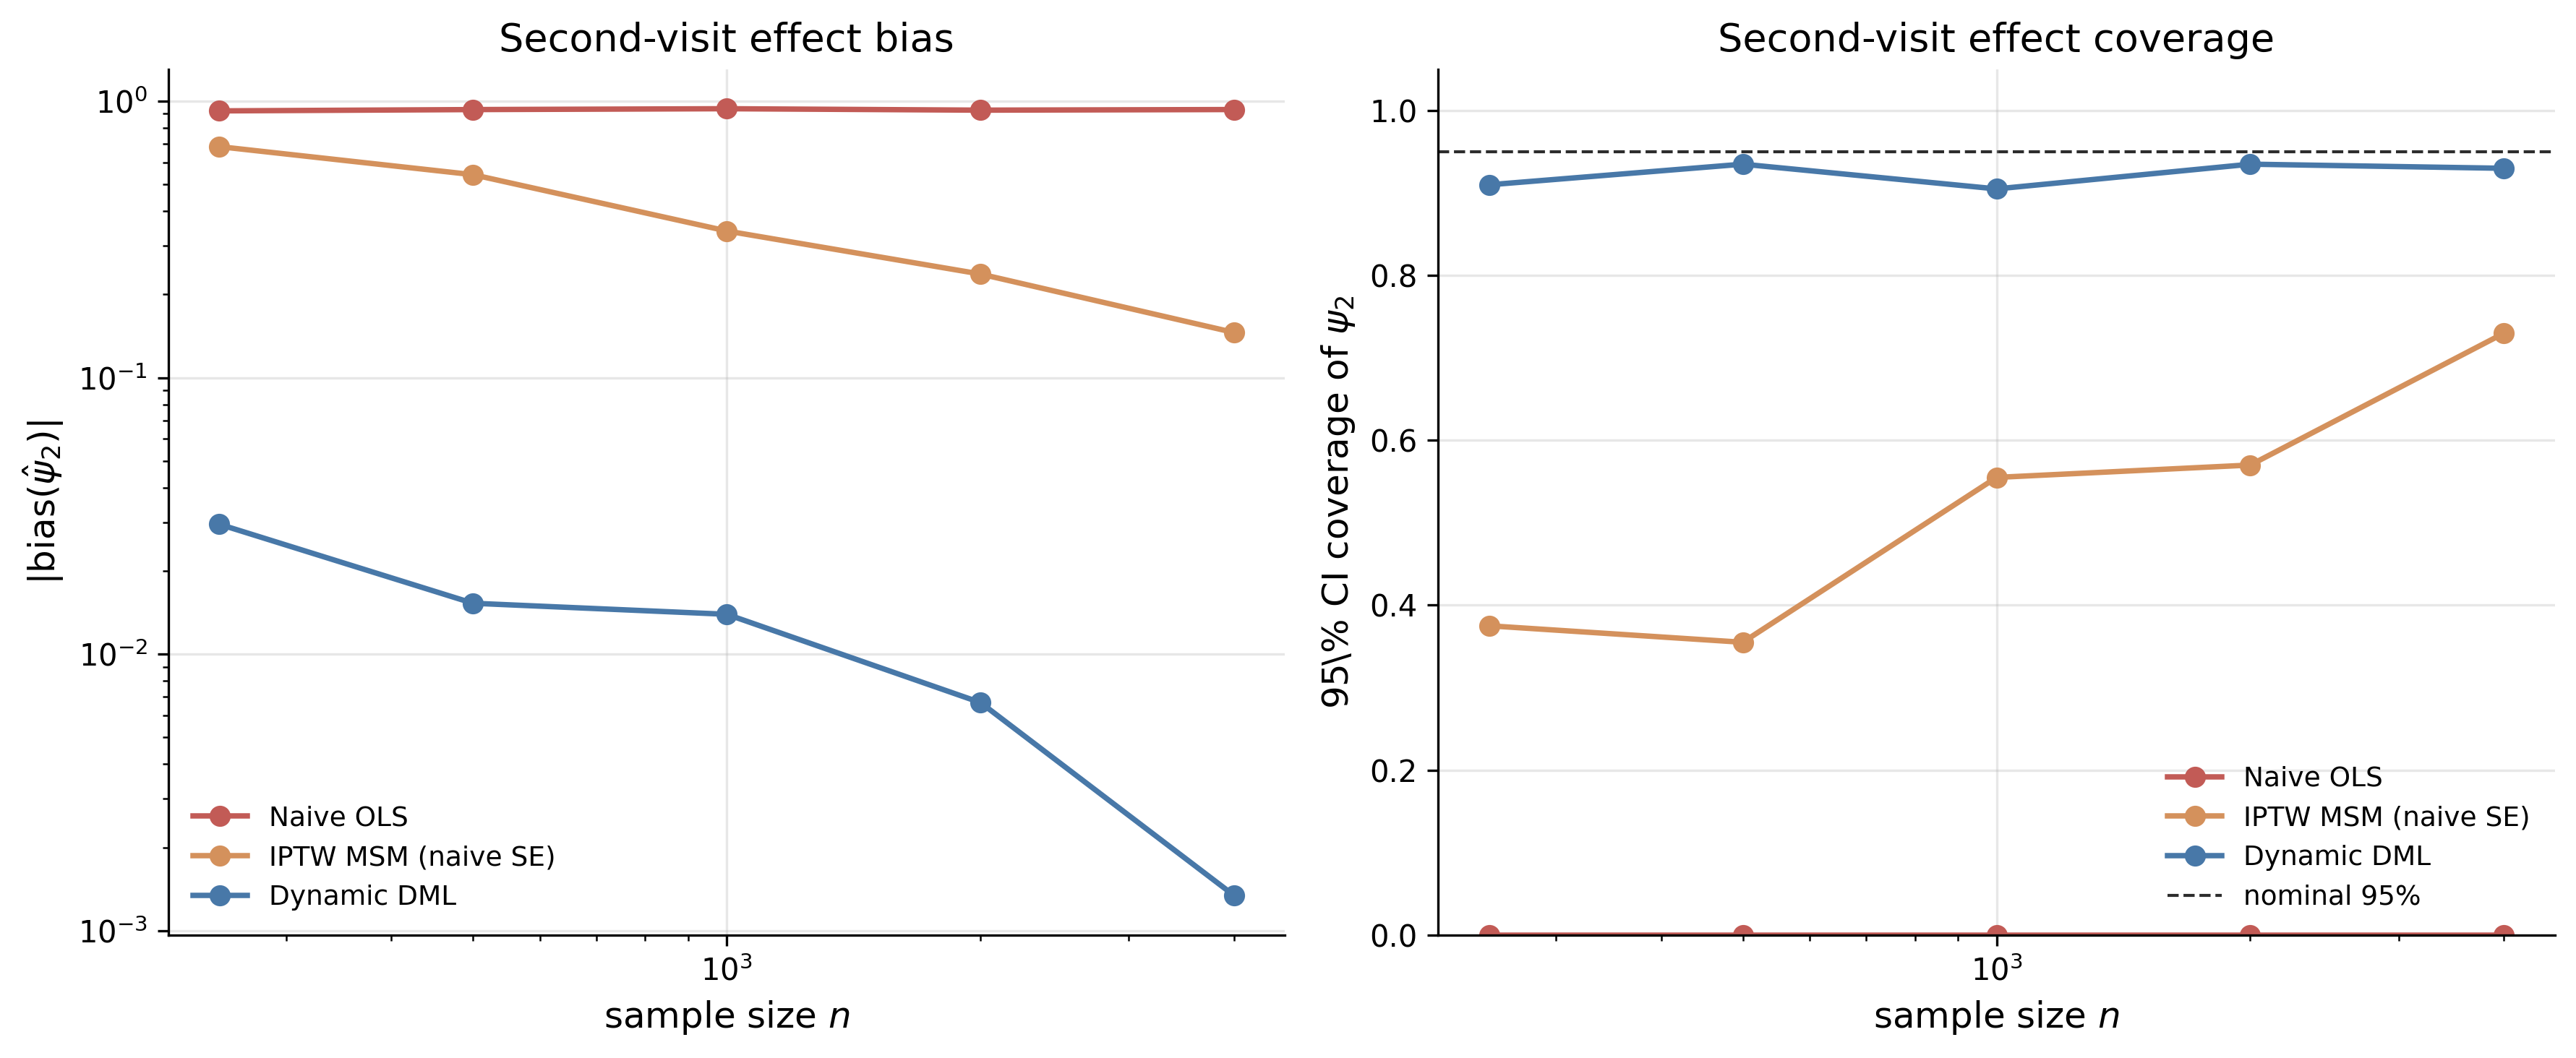
\includegraphics[width=\textwidth]{../ch10b_rl_for_ci/sims/dynamic_dml_snmm_coverage.png}
\caption{Sim 2, dynamic DML on a two-stage SNMM. Left panel: absolute bias of $\hat\psi_2$ versus sample size $n$ (log-log). Right panel: empirical coverage of nominal $95\%$ confidence intervals on $\psi_2$ versus $n$. Dotted reference line is the nominal coverage level. Each point averages 200 Monte Carlo replications under the data-generating process in Equation~\eqref{eq:simB1_dgp}.}
\label{fig:simB1}
\end{figure}

Both simulations corroborate the theoretical claims of the underlying papers. Sim~1 shows that on a correctly specified tabular problem every estimator in the canon recovers the dynamic-programming truth, that the horizon behavior separates the trajectory-weighted estimators from the marginalized one exactly as \citet{liu2018curse} and \citet{xie2019marginalized} predict, and that the double-robustness pattern of \citet{jiangli2016doubly} appears cell-for-cell in the misspecification design. Sim~2 shows that the Lewis-Syrgkanis recursive residualisation moment delivers the $\sqrt n$ asymptotic normality predicted by Theorem~4 of \citet{lewisSyrgkanis2021dynamicDML}, even though the state is high-dimensional, the propensities are confounded, and naive panel regression with the same nuisance learners is biased. The chapter's broader thesis is that this is standard machine-learning machinery brought to bear on a dynamic causal-inference recursion, under the identification assumptions catalogued in Section~\ref{subsec:gmethods_bridge}.

%%%%%%%%%%%%%%%%%%%%%%%%%%%%%%%%%%%%%%%%%%%%%%%%%%%%%%%%%%%%%%%%%%%%%%%%%%%%%%%
\subsection{Discussion}
\label{subsec:rl_for_ci_discussion}
%%%%%%%%%%%%%%%%%%%%%%%%%%%%%%%%%%%%%%%%%%%%%%%%%%%%%%%%%%%%%%%%%%%%%%%%%%%%%%%

The sections of this chapter share one underlying claim. Dynamic causal inference and reinforcement learning are the same enterprise applied to different data sources, not separate enterprises that happen to use similar notation. The recursion in Section~\ref{subsec:gmethods_bridge} is Bellman's. The doubly robust OPE score of Section~\ref{subsec:ope} is in the same family as the augmented inverse-propensity estimators of the Robins tradition, applied stage by stage through the horizon. The Lewis-Syrgkanis sequential residualisation is Robins's g-estimation with cross-fitting added. The Sakaguchi backward-induction AIPW is the offline-RL Q-learning update with doubly-robust scoring. In each case the move is not to invent a new algorithm but to recognize that an algorithm developed in one tradition addresses a question that arose in the other tradition.

Three implications follow for the empirical worker.

First, the rate of convergence of an estimator is determined by the orthogonality of the moment that defines it, not by the field in which the moment was first written down. The orthogonal statistical learning theory of \citet{fosterSyrgkanis2023orthogonal} unifies the dynamic-DML rate calculations of Section~\ref{subsec:dml_dte} with the policy-learning regret bounds of Section~\ref{subsec:dynamic_offline_policy}. The common requirement is that nuisance estimation errors enter the target estimator at second order; the common consequence is that any sufficiently fast machine learner can be used for the nuisance components without sacrificing the parametric rate on the structural target. This is the modern semiparametric efficiency story, transported into reinforcement learning territory.

Second, identification is prior to estimation. The recursions in this chapter all rely on sequential ignorability, positivity, and consistency. When those assumptions hold by design (a sequential multiple-assignment randomized trial, an adaptive field experiment with a known assignment mechanism, a known causal graph), the chapter's techniques deliver $\sqrt n$ inference on dynamic causal quantities. When they fail, the recursions still run but they no longer estimate causal quantities; the proxy, instrument, sensitivity, and mediator strategies of Chapter~\ref{section:causal_rl} are the recovery routes. The economist's instinct to ask first what identifies the parameter of interest, then what estimates it, applies unchanged here.

Third, the bridge runs in both directions. Several of the most useful results in modern reinforcement learning are descendants of biostatistical and econometric reasoning rather than purely computer-scientific. The advantage doubly-robust estimator of \citet{nie2021whentotreat} is the dynamic generalization of the Athey-Wager policy-learning estimator. The recursive Riesz representers of \citet{chernozhukov2023automatic} are an automation of the locally-robust correction that Robins introduced in g-estimation. The traffic of ideas is two-way, and a chapter framed as ``reinforcement learning for causal inference'' could equally be read as ``causal inference recovers, validates, and extends reinforcement learning under identification.''

Open problems remain in several directions. The dynamic-DML rate of \citet{lewisSyrgkanis2021dynamicDML} is established for parametric structural nested mean models with linear blips; extensions to fully nonparametric blip functions, to the high-stake combination of large state spaces and adaptively collected data, and to settings where the policy class itself is learned from the data (rather than pre-specified) are active research topics. Each of these open problems is, at the methodological level, a question about how to import additional machine-learning machinery into a causal-inference recursion without losing the orthogonality property that makes the rate work.

A final remark on practice. The Tennessee Project STAR re-analysis of \citet{sakaguchi2024dynamicpolicy} and the Japanese energy-rebate experiment of \citet{idaIshiharaItoEtAl2024energyrebate} are the chapter's clearest demonstrations that the theory has practical purchase: doubly-robust backward induction applied to real cohorts delivers dynamic regimes with measured welfare gains. The chapter's broader message is that this combination is no longer exotic. It is the natural next step once one accepts that dynamic causal inference and reinforcement learning are doing the same thing under different names, and that the modern machine-learning toolkit, applied carefully, can serve both at once.
